\subsection{Оптимизация запросов. Выбор методов исполнения запроса}

\begin{definition}
	\textit{Сеть операций} -- граф вычислений запросов в реляционной алгебре. Аргументы для каждого
	узла -- базовые таблицы или результаты других операций, результат узла является либо аргументом
	другого узла.
\end{definition}

В графе выделяют два типа  узлов:

\begin{itemize}
	\item \textbf{Преобразователи} -- просматривают аргументы в процессе работы и не хранят
	      информацию в памяти. Другими словами, из таких операций записи можно получать по одной записи.
	      Используют внутри себя курсоры.
	\item \textbf{Контейнеры} -- загружают аргументы, сохраняют результаты, при необходимости -- на
	      диске. В отличие от преобразователей требуют все входные данные вместе для выполнения операции.
\end{itemize}

Пример сети операций приведен на рисунке \ref{operation-network}. Синим цветом отмечены
преобразователи, зеленым -- контейнеры.

\begin{figure}[H]
	\centering
	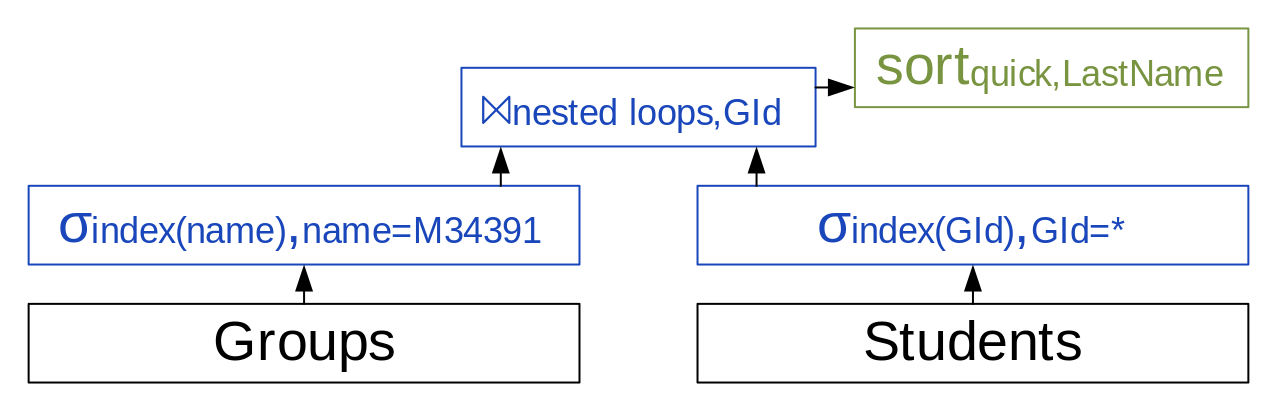
\includegraphics[width=0.8\textwidth]{../assets/kgeorgiy/optimization/Network_Students_Types.svg.png}
	\caption{Пример сети операций}
	\label{operation-network}
\end{figure}

\paragraph{Унарные операции}

\begin{itemize}
	\item \textbf{Фильтрация}. Преобразователь. игнорирует строки, не удовлетворяющие условию.
	      \begin{itemize}
		      \item \textit{Трудоемкость}: $\mathcal{O}(n)$, где $n$ -- размер входных данных;
		      \item \textit{Свойства}: Операция может существенно уменьшать количество обрабатываемых
		            строк, что учитывается в планировщике путем оценки селективности.
	      \end{itemize}
	\item \textbf{Проекция}. Преобразователь. В случае, если указан \texttt{distinct}, удаляет
	      дубликаты по проецируемым атрибутам, иначе только помечает, какие атрибуты больше не требуются.
	      \begin{itemize}
		      \item \textit{Трудоемкость}: $\mathcal{O}(n)$, где $n$ -- размер входных данных;
		      \item \textit{Свойства}: данные на входе должны быть упорядочены, результат операции
		            сохраняет порядок.
	      \end{itemize}
	\item \textbf{Сортировка}. Контейнер. Если данные помещаются в оперативную память, производится
	      сортировку в ней, иначе применяется внешняя сортировка, которая значительно менее производительна.
	      \begin{itemize}
		      \item \textit{Трудоемкость}: $\mathcal{O}(n \log(n))$, где $n$ -- размер входных данных;
		      \item \textit{Свойства}: результат операции -- упорядоченные данные, время исполнения
		            скачкообразно зависит от объема входных данных (скачок происходит при аллокации новой памяти).
	      \end{itemize}
	\item \textbf{Просмотр таблиц}. В зависимости от реализации -- преобразователь (полный проход
	      по таблице) или контейнер (выдача в отсортированном виде).
	      \begin{itemize}
		      \item \textit{Трудоемкость}: $\mathcal{O}(n)$, где $n$ -- размер входных данных;
		      \item \textit{Методы исполнения}: полный просмотр, использование индекса,
		            использование кластеризованного индекса.
	      \end{itemize}
\end{itemize}

\paragraph{Множественные операции}

\begin{itemize}
	\item \textbf{Объединение}. Преобразователь. Производит слияние двух аргументов.
	      \begin{itemize}
		      \item \textit{Трудоемкость}: $\mathcal{O}(n)$, где $n$ -- размер входных данных;
		      \item \textit{Свойства}: ожидается, что аргументы упорядочены, результат также будет
		            упорядочен.
	      \end{itemize}
	\item \textbf{Пересечение}. Полностью аналогично объединению.
	\item \textbf{Разность}. Полностью аналогично объединению.
\end{itemize}

\paragraph{Соединения}

Существует несколько подходов построения соединений.

\begin{itemize}
	\item \textbf{Вложенный перебор}. Преобразователь. Для каждой строки левого аргумента ищет
	      строку из правого аргумента полным перебором.
	      \begin{itemize}
		      \item \textit{Трудоемкость}: $\mathcal{O}(l \cdot r)$, где $l$, $r$
		            -- размеры левого и
		            правого аргументов;
		      \item \textit{Свойства}: сохраняет упорядоченность (по столбцам левого аргумента, при
		            равенстве левого аргумента -- по столбцам правого).
	      \end{itemize}
	\item \textbf{Поиск по дереву}. Преобразователь. Для каждой строки левого аргумента ищет
	      строку из правого аргумента с помощью индекса. Применим если уже построен индекс методом дерева.
	      \begin{itemize}
		      \item \textit{Трудоемкость}: $\mathcal{O}(\max(l \cdot \log(r), n))$, где $l$, $r$
		            --
		            размеры левого и правого аргументов, $n$ -- размер выхода;
		      \item \textit{Свойства}: сохраняет упорядоченность (аналогично вложенному перебору).
	      \end{itemize}
	\item \textbf{Поиск по хешу}. Преобразователь и контейнер. Перед соединением правый аргумент
	      хешируется. Для каждой строки левого аргумента ищет строку из правого аргумента с помощью хеша.
	      Если хеш-индекс уже построен, может переиспользовать его.
	      \begin{itemize}
		      \item \textit{Трудоемкость}: $\mathcal{O}(\max(l + r, n))$, где $l$, $r$
		            --
		            размеры левого и правого аргументов, $n$ -- размер выхода.
	      \end{itemize}
	\item \textbf{Слияние}. Преобразователь. Применим если входные аргументы упорядочены по общим
	      атрибутам. Производится стандартным алгоритмом слияния.
	      \begin{itemize}
		      \item \textit{Трудоемкость}: $\mathcal{O}(\max(l + r, n))$, где $l$, $r$
		            --
		            размеры левого и правого аргументов, $n$ -- размер выхода;
		      \item \textit{Свойства}: требует упорядоченности аргументов, сохраняет упорядоченность.
	      \end{itemize}
\end{itemize}
